\chapter{Модуль алгебраической декомпозиции}\label{ch:algdec}

Данная глава посвящена описанию работы модуля алгебраической декомпозиции, особенностей реализации.

\section{Описание алгоритма}
Работа алгоритма начинается с того, что для каждого из уравнений генерируемой на среднем уровне СНАУ вычисляется набор переменных от которого это уравнение зависит. Вывод переменных зависимости реализуется вручную, путём анализа каждого уравнения. В итоге, получив для каждого уравнения набор переменных, от которых оно зависит, можно построить двудольный граф, который и будет непосредственно участвовать в декомпозиции. Вершинами такого графа являются уравнения и переменные, которые и образуют две доли, а ребро между вершиной-уравнением $y$ и вершиной-переменной $x$ существует тогда, когда уравнение $y$ зависит от переменной $x$. Пример такого графа изображен на рисунке \ref{fig:graph_example}. В дальнейшем, над таким графом выполняется ряд преобразований, который разбивает граф на несколько подграфов, которые соответствуют подсистемам уравнений, которые можно решать по отдельности. 

\begin{figure}[h]
	\centering
	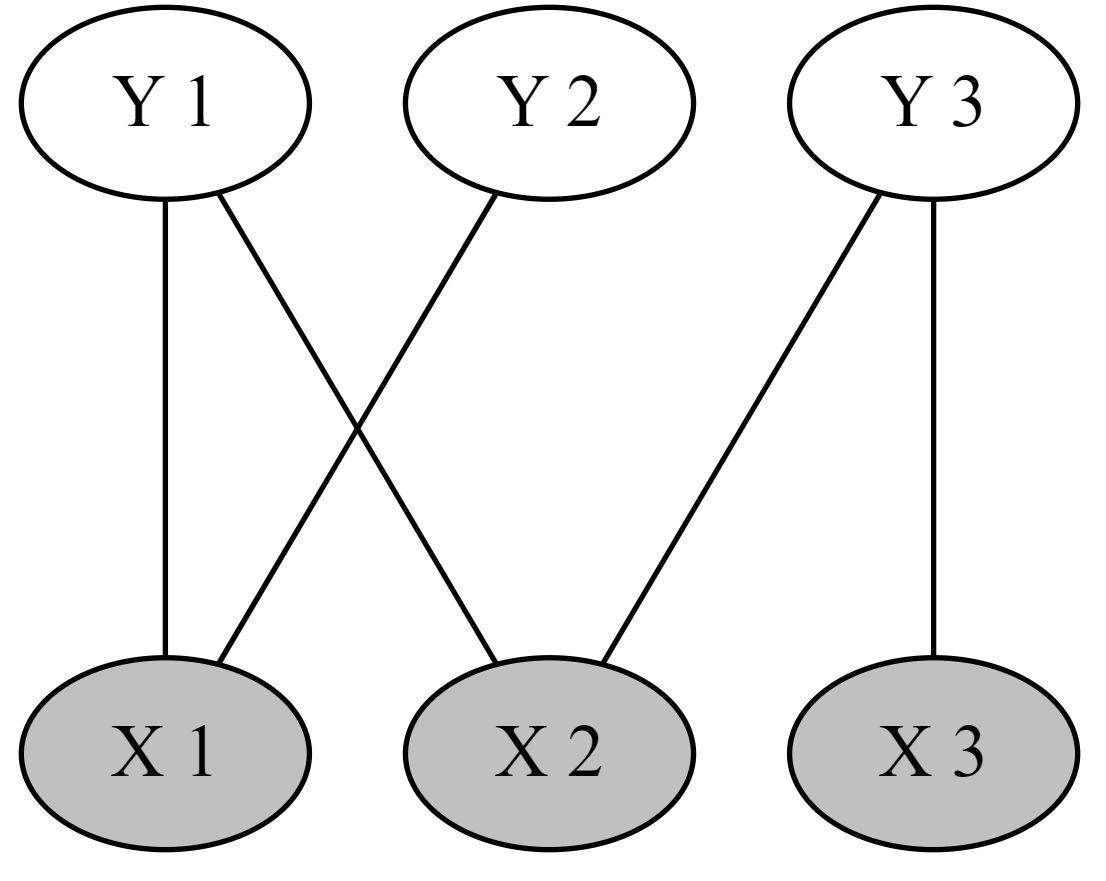
\includegraphics[width=0.3\linewidth]{fig_graph_example.png}
	\caption{Пример графа зависимости уравнений от переменных в системе}
	\label{fig:graph_example}
\end{figure}

Работа алгоритма разделена на две основных части. Сначала производится разделение графа на три подграфа (как минимум один из которых не является пустым) соответствующих пере-, недо- и хорошо-определенным подсистемам. \textit{Хорошо определенной системой} называется такая система уравнений, в графе которого существует идеальное паросочетание. Система уравнений называется \textit{переопределённой}, если число уравнений в ней больше чем число переменных, и наоборот если число переменных меньше числа уравнений, то система называется \textit{недоопределённой} \cite{ait2014reduction}. После первого этапа, если граф хорошо-определённой подсистемы не пуст, то он разбивается на множество хорошо-определённых несократимых подсистем. Несократимость подсистемы означает невозможность разделить подсистему тем же алгоритмом, или же математически это свойство записывается как условие, что для любого подмножества вершин уравнений $Y'$ из уравнений $Y$ выполняется:
\begin{equation*}
 \left|\Gamma(Y') \right| > \left|Y'\right|
\end{equation*}
где: $\Gamma(Y)$ -- множество соседей вершин $Y$, $ \left|Y\right|$ -- мощность множества $Y$.

Второй этап декомпозиции хорошо-определенной подсистемы существенно опирается на предположение о том, что любая хорошо-определённая система имеет хотя бы одно решения. Но в общем случае это не верно, но на практике эффект этого явления слабее чем достигаемое ускорение. В случае не успешного решения одной из подсистем, можно попытаться решить исходную систему уравнений целиком. В таком случае, алгебраическая декомпозиция не уменьшит процент успешно решённых тестов, но ускорение обеспечиваемое декомпозицией также станет меньше, в зависимости от числа тестов, в которых одна из подсистемы была решена не успешно. 

\section{Устройство алгоритма}

Для полного описания обоих частей алгоритма, необходимо ввести следующее преобразование графа $K$:

\textbf{Определение.} Пусть дан граф неориентированный двудольный $G$ и его максимальное паросочетание $M$. Тогда преобразование $K$ переводит граф $G$ в ориентированный двудольный граф $G'$, путём замены всех рёбер из паросочетания $M$ на две дуги $xy$ и $yx$, и ориентированием всех не попавших в паросочетание рёбер от $Y$ к $X$, где $X$ -- вершины-переменные, $Y$ -- вершины-уравнения.

Используя это определение, устройство первой части алгоритма можно записать следующим образом, обозначая исходный граф системы как $G$, граф хорошо-определённой подсистемы как $G_1$,  переопределённой  -- $G_2$, недоопределённой -- $G_3$ \cite{ait2014reduction}:
\begin{enumerate}
    \item 
        Найти максимальное паросочетание $M$ в $G$.
    \item
        Получить ориентированный граф $G'$, применив преобразование $K$ к графу $G$.
    \item
        $G_2$ -- это множество всех потомков от всех истоков в графе $G'$.
    \item
        $G_3$ -- это множество всех предков от всех стоков в графе $G'$.
    \item
        В итоге $G_1 = G - G_2 - G_3$ 
\end{enumerate}
Шаги алгоритма 2--5 могут быть выполнены за время $O(|X| + |Y|)$. А весть алгоритм может быть выполнен за время оцениваемое как $O(|Y|\cdot |X|^\frac{1}{2})$ с использованием алгоритма Хопкрофта — Карпа на шаге 1 \cite{hopcroft1973n}. Важно отметить, что подсистемы $G_2$ и $G_3$ могут содержать в себе несколько независимых компонент. Поэтому имеет смысл также анализировать эти подсистемы, и разбивать их на независимые части. Полученные подсистемы должны решаться в следующем порядке: $G_2, G_1, G_3$.

Вторая часть алгоритма, разбивает подсистему $G_1$ на набор несократимых подсистем, и устроена она следующим образом:
\begin{enumerate}
    \item 
        Найти максимальное паросочетание $M_1$ в $G_1$ (для этого можно использовать уже найденное ранее паросочетание M).
    \item
        Построить ориентированный граф $G_1'$ применяя преобразование $K$ к графу $G_1$.
    \item
        Найти в $G_1'$ компоненты сильной связности $S$, которые и являются несократимыми подсистемами.
    \item
        Для определения порядка решения подсистем из $S$ необходимо произвести топологическую сортировку компонент $S$. Порядок заданный сортировкой, определяет порядок решения систем.
\end{enumerate}
Шаги 2 -- 4 могут быть вычислены за $O(|X| + |Y|)$, с использованием алгоритма Тарьяна \cite{tarjan1972depth} для шагов 3 -- 4, поскольку этот алгоритм гарантирует, что все компоненты в $S$ будут отсортированы.

\textcolor{red}{\textbf{TODO: описать особенности работы с уравнением BoundedValue}}